\documentclass[11pt]{article}
\usepackage[margin=2.5cm]{geometry}
\usepackage[T1]{fontenc}
\usepackage{amsmath}
\usepackage[round]{natbib}
\usepackage[colorlinks=true,linkcolor=blue,citecolor=blue,urlcolor=blue]{hyperref}
\usepackage{graphicx}
\usepackage{microtype}
\usepackage{booktabs}
\usepackage{tikz}
\usetikzlibrary{arrows.meta}

\setlength{\bibsep}{0pt}

\title{Direct One-Shot Forecasts and Respondent-Twin Simulations of Experimental Effects\\
\large A comparison on 469 archived contrasts}
\author{GPT-6-Luna Guided by John Horton\\\small MIT Sloan, NBER and Expected Parrot}
\date{}

\begin{document}
\maketitle
\newcommand{\TwinsMAE}{0.0735}
\newcommand{\BestSingleMAEMin}{0.0551}
\newcommand{\BestSingleMAEMax}{0.0560}
\newcommand{\MeanOneShotMAE}{0.0532}
\newcommand{\MeanOneShotGain}{0.0202}
\newcommand{\MeanTwinDeltaLow}{-0.0327}
\newcommand{\MeanTwinDeltaHigh}{-0.0080}
\newcommand{\TwinSignAccuracyPct}{69}
\newcommand{\MeanOneShotSignAccuracyPct}{70}
\newcommand{\BestSingleGain}{0.0019}
\newcommand{\WeightedMAE}{0.0535}
\newcommand{\EqualMAE}{0.0532}
\newcommand{\WeightedEqualLow}{-0.0004}
\newcommand{\WeightedEqualHigh}{0.0010}
\newcommand{\AstraFoldWeight}{0.1808}
\newcommand{\ClaudeFoldWeight}{0.3393}
\newcommand{\GeminiFoldWeight}{0.4799}


\begin{abstract}
Language models can forecast an experiment by simulating respondents and aggregating their answers, or by predicting the treatment effect directly. We compare the archive's GPT-4 respondent-twin estimates \cite{ashokkumar2026predict} with one-shot forecasts from three frontier models on 469 contrasts across 70 social-science experiments. Direct forecasts have lower mean absolute error (MAE), and their equal-weight average performs best among evaluated forecasts; study-held-out weights add no improvement. The one-shot mean has lower MAE in all five groups defined by observed effect magnitude, with a small difference for the smallest effects and larger gains for larger effects. Because model generations and prompts differ, this comparison evaluates systems rather than isolating respondent simulation's value. A prospective, model-matched test is needed.
\end{abstract}

\section{Introduction}
Language models are increasingly used to anticipate human responses before an experiment is run. One strategy creates a sample of simulated participants, asks each to respond under the experimental conditions, and aggregates those responses. A second strategy gives a model the study description and asks it to predict the aggregate contrast directly. The first resembles a synthetic pilot; the second resembles a forecast. If the goal is an average treatment effect, the extra respondent simulation may or may not buy useful accuracy.

Research has shown that language models can reproduce some human-subject findings and generate samples with meaningful demographic variation \citep{argyle2023out,aher2023simulate}. Work on experimental forecasting has also evaluated direct predictions of study outcomes, while survey-simulation research examines how well language models reproduce response distributions \citep{ashokkumar2026predict,cao2025specializing}. These approaches answer related but distinct questions. A distribution over individual responses can matter for subgroup analysis, mechanisms, or outcome distributions. For forecasting a single average contrast, however, a direct prediction may be a more economical competitor.

The comparison builds directly on the experimental archive and simulated-response forecasts assembled by Ashokkumar et al. \citep{ashokkumar2026predict}. \textbf{This note asks:} Do respondent twins improve forecasts of aggregate experimental effects relative to direct one-shot predictions? It reuses the original human outcomes and GPT-4 twin estimates, then adds direct forecasts from newer models for the same contrasts. It is therefore a reanalysis and extension of Hewitt and colleagues' benchmark, not an independent replication. Because the forecast systems and prompts differ, the comparison evaluates their practical performance in this archive rather than isolating the causal contribution of respondent simulation.

\section{Forecasting strategies and evaluation}
\subsection{Two routes to an effect forecast}
Let $A$ and $B$ denote the first- and second-listed experimental conditions, and let $\tau=\bar{Y}_B-\bar{Y}_A$ be the observed difference in their mean outcomes. A respondent-twin procedure simulates answers for participants under each condition, aggregates within condition, and subtracts the two aggregates. A one-shot procedure reads the study prompt and predicts $\tau$ directly. Figure~\ref{fig:paths} depicts the distinction. Both produce an estimate of the mean contrast, but only the twin route also produces respondent-level answers.

\begin{figure}[t]
\centering
\begin{tikzpicture}[
  x=1in, y=1in,
  box/.style={draw, rounded corners=2pt, align=center, inner sep=4pt,
    minimum height=0.38in, font=\small},
  lane/.style={box, text width=1.25in, fill=gray!8},
  processbox/.style={box, text width=2.15in, fill=blue!4},
  result/.style={box, text width=1.2in, fill=orange!7},
  flow/.style={-{Stealth[length=1.7mm]}, line width=0.6pt}
]
\node[lane] (twin) at (0.70,0.30) {Respondent twins};
\node[processbox] (simulate) at (2.88,0.30) {Simulate answers in $A$ and $B$; aggregate each condition};
\node[result] (twinout) at (5.13,0.30) {Twin forecast $\hat{\tau}_T$};
\node[lane] (shot) at (0.70,-0.30) {One-shot forecast};
\node[processbox] (direct) at (2.88,-0.30) {Read the study description; predict $B-A$ directly};
\node[result] (shotout) at (5.13,-0.30) {Direct forecast $\hat{\tau}_S$};
\draw[flow] (twin) -- (simulate);
\draw[flow] (simulate) -- (twinout);
\draw[flow] (shot) -- (direct);
\draw[flow] (direct) -- (shotout);
\end{tikzpicture}
\caption{The procedures differ in how they reach a forecast; both are scored against the same observed mean contrast.}
\label{fig:paths}
\end{figure}

\subsection{Benchmark and extension}
Ashokkumar et al. assembled 70 preregistered, nationally representative United States survey experiments and used GPT-4 to simulate demographically profiled respondents answering the original experimental stimuli; averaging simulated responses within conditions yielded the twin treatment-effect estimates \citep{ashokkumar2026predict}. The present analysis reuses the 469 contrasts in that archive for which both human outcomes and original GPT-4 estimates are available. It adds one-shot predictions from GPT-6 Astra, Claude Fable 5, and Gemini 4 Argon: each receives selected survey prompts for the two conditions and directly predicts their mean difference, without generating respondent profiles or aggregating simulated answers. We score all approaches on the same observed contrasts using absolute error and sign accuracy. Uncertainty calculations resample experiments, retaining their nested contrasts.

\subsection{Scores and combinations}
We report mean absolute error, $\mathrm{MAE}=n^{-1}\sum_i|\hat{\tau}_i-\tau_i|$, and sign accuracy, the share of forecasts with the correct direction. The primary comparison uses absolute error because a useful forecast should be close in magnitude as well as direction. We evaluate the equal-weight mean of the three one-shot predictions. We also fit nonnegative weights summing to one to minimize absolute error, separately for each held-out study using all other studies. This leave-one-study-out procedure prevents an observation from helping choose its own weights. Confidence intervals for paired MAE differences use a cluster bootstrap that resamples the 70 studies and retains all contrasts within each sampled study.

\section{Results}
\subsection{Aggregate accuracy}
The individual one-shot models have MAEs between \BestSingleMAEMin{} and \BestSingleMAEMax{}, compared with \TwinsMAE{} for the archived respondent twins (Table~\ref{tab:main}). The equal-weight one-shot mean reaches \MeanOneShotMAE{}, a reduction of \MeanOneShotGain{} outcome units relative to the twins. Its study-cluster bootstrap interval for the paired MAE difference is $[\MeanTwinDeltaLow{},\MeanTwinDeltaHigh{}]$, where negative values favor the one-shot mean. The one-shot models' sign accuracy is about \MeanOneShotSignAccuracyPct{}\%, close to the twins' \TwinSignAccuracyPct{}\%. The advantage is therefore mainly about distance from the observed effect, not a dramatic improvement in identifying its direction.

\begin{table}[t]
\centering
\small
\caption{Forecast performance on 469 contrasts in 70 studies. Lower MAE is better.}
\label{tab:main}
\begin{tabular}{lrrr}
\toprule
Forecast & MAE & RMSE & Sign accuracy \\
\midrule
Original GPT-4 respondent twins & 0.0735 & 0.1071 & 0.691 \\
GPT-6 Astra, one-shot & 0.0560 & 0.0766 & 0.706 \\
Claude Fable 5, one-shot & 0.0556 & 0.0819 & 0.701 \\
Gemini 4 Argon, one-shot & 0.0551 & 0.0811 & 0.697 \\
Equal mean of one-shots & 0.0532 & 0.0762 & 0.699 \\
Study-held-out weighted mean & 0.0535 & 0.0776 & 0.708 \\
\bottomrule
\end{tabular}

\end{table}

\subsection{Performance across effect magnitudes}
Table~\ref{tab:magnitude} shows contrast-level MAEs by fifth of observed effect magnitude. The one-shot mean has lower MAE in all five groups; the difference is small for the smallest effects and increases across the larger-effect groups. These bins are descriptive and should not be read as a pre-registered subgroup test.

\begin{table}[t]
\centering
\small
\caption{MAE by fifth of observed effect magnitude. The bins contain approximately equal numbers of contrasts.}
\label{tab:magnitude}
\begin{tabular}{lrrr}
\toprule
Observed $|\tau|$ fifth & $n$ & Equal one-shot MAE & Twin MAE \\
\midrule
Smallest & 94 & 0.0345 & 0.0372 \\
Second & 94 & 0.0328 & 0.0440 \\
Middle & 93 & 0.0476 & 0.0717 \\
Fourth & 94 & 0.0650 & 0.0942 \\
Largest & 94 & 0.0862 & 0.1201 \\
\bottomrule
\end{tabular}

\end{table}

\subsection{Combining one-shot forecasts}
Averaging three frontier forecasts improves MAE by about \BestSingleGain{} relative to the best single model. This is consistent with small complementary errors, although the improvement is modest. Study-held-out weights average \AstraFoldWeight{} for GPT-6 Astra, \ClaudeFoldWeight{} for Claude Fable 5, and \GeminiFoldWeight{} for Gemini 4 Argon across folds. The weighted forecast's MAE is \WeightedMAE{}, slightly worse than equal weighting at \EqualMAE{}. The cluster-bootstrap interval for weighted-minus-equal MAE is $[\WeightedEqualLow{},\WeightedEqualHigh{}]$, so these data do not establish a useful advantage for estimating weights. A simple mean is the more defensible combination here.

To show the individual contrasts that study averages conceal, Figure~\ref{fig:studygrid} facets all 469 comparison paths by experiment. The small panels make this a diagnostic overview rather than a print-scale summary; the full-size companion figure can be enlarged to inspect individual experiments.

\clearpage
\begin{figure}[p]
\centering
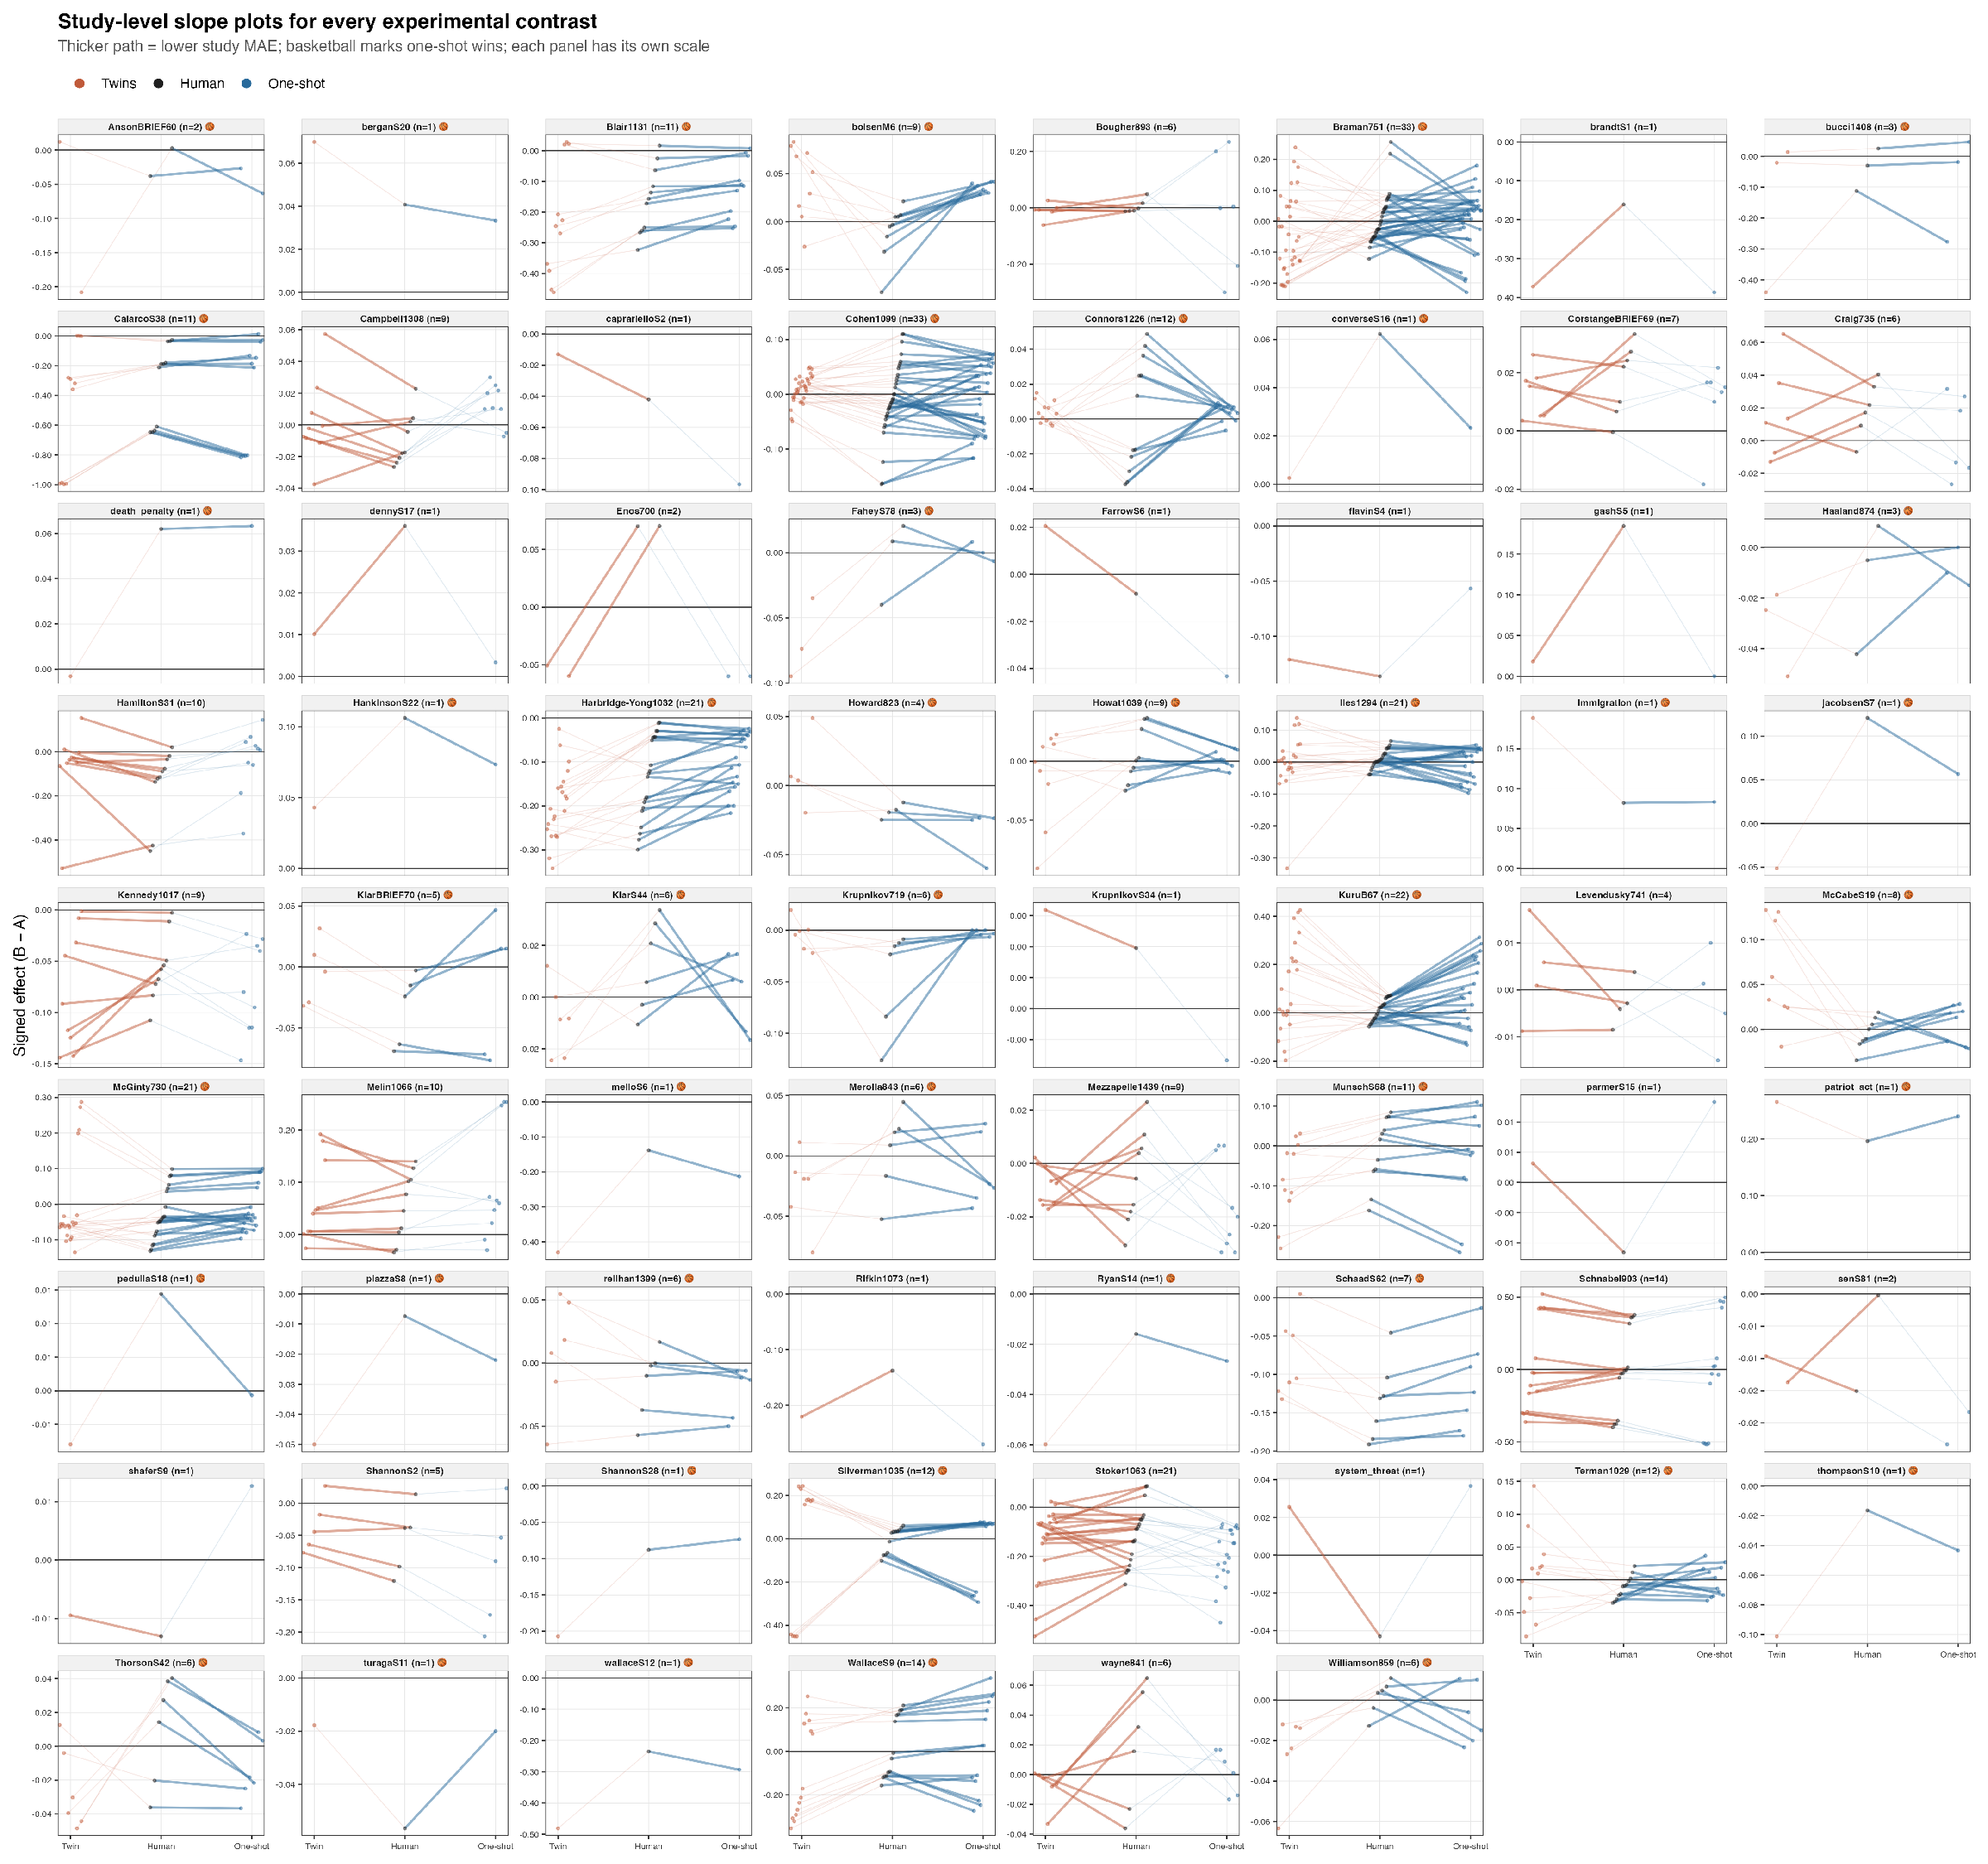
\includegraphics[width=0.99\textwidth,height=0.76\textheight,keepaspectratio]{study_slope_grid.pdf}
\caption{All 469 contrast-level slope paths, faceted by experiment (70 panels; the final two grid cells are empty). Within each experiment, contrasts are ranked by observed human effect and evenly spread across a small horizontal jitter band; each contrast's three estimates share the same offset. Paths connect the original respondent-twin estimate, the observed human contrast, and the mean one-shot estimate. Color separates twin-to-human from human-to-one-shot segments; horizontal reference lines mark zero. Within each panel, the thicker segment identifies the method with lower mean absolute error across that study's contrasts; a basketball marks one-shot wins. Each panel has an independent vertical scale, so slopes and magnitudes are comparable within a study but not across studies.}
\label{fig:studygrid}
\end{figure}
\clearpage

\section{Interpretation and limitations}
The comparison suggests that respondent simulation is not necessary for producing competitive point forecasts of average experimental effects in this archive. A direct prompt can reach the target with lower average absolute error and less intermediate machinery. But the result is about the evaluated systems, not the simulation step in isolation. The respondent twins were generated with GPT-4; the direct forecasts use later models. The prompting procedures and available study descriptions also differ. Improvements could reflect model capability, prompt design, forecast target alignment, or simulation itself. A matched comparison would hold the model and study information fixed while varying whether it predicts the contrast directly or predicts and aggregates participant responses.

The result also concerns aggregate contrasts only. Respondent-level simulation may still be valuable when researchers need subgroup forecasts, response distributions, heterogeneity, or an auditable account of how an aggregate prediction arises. This evaluation does not test those uses. Nor does lower archive MAE show that either method can replace human pilot data or predict results for new populations and settings. The archive contains repeated contrasts within studies, and its 70 studies are a limited basis for claims about transport to other research domains. The cluster bootstrap addresses within-study dependence in uncertainty, but it cannot make the set of studies representative.

There is a consequential difference in what the methods return. A one-shot forecast supplies a point estimate for the specified contrast; by construction, it does not identify how outcomes covary across people or conditions. Twin simulations retain respondent-level answers and can estimate joint distributions when respondent identities are linked across conditions or questions, supporting analyses of heterogeneity and mechanisms as well as the mean effect. This is the broader computational-agent use proposed by the \emph{Homo silicus} perspective \citep{horton2023homosilicus}. Such distributions are not automatically human-valid: they need to be checked against observed response distributions and can potentially be improved through better respondent profiles, prompts, sampling, and calibration. This comparison evaluates only mean-effect accuracy, so it provides no evidence about which method better recovers joint distributions.

The magnitude breakdown offers a useful lead rather than an explanation. Direct forecasts have their clearest advantage among larger observed effects, while the two approaches are essentially tied near zero. One possible account is that the twins' aggregation procedure compresses or distorts some study-level contrasts; another is that newer models recognize study-level cues that the earlier twin system misses. The present data cannot separate these mechanisms. A prospective evaluation should register a set of new experiments, create both forecasts before outcomes are observed, use the same model family and study materials for both routes, and report both aggregate and distributional scores.

\section{Conclusion}
On 469 archived contrasts, direct one-shot forecasts outperform the original respondent twins on mean absolute error, and equal averaging of three one-shots performs slightly better still. For an aggregate point forecast, the one-shot route is a strong and simpler baseline; it does not replace the respondent-level joint distributions that twins can generate, whose validity and potential for improvement remain open questions. A prospective, model-matched comparison should evaluate both aggregate accuracy and distributional fidelity.

\bibliographystyle{abbrvnat}
\bibliography{refs}
\end{document}
